%%%%%%%%%%%%%%%%%%%%%%%%%%%%%%%%%%%%%%%%%%%%%%%%%%%%%%%%%%%%%%%%%%%%%%%%%%%%%%%%
\chapter{Overall System Design}
\label{chap:system_design}

The RANPilotAI platform adopts a modular software architecture in which four independent analytical modules operate within a unified web-based engineering environment. Rather than implementing a monolithic application, the platform separates domain-specific analytical processing from common infrastructure services, ensuring that each module can be developed, tested, and deployed independently while presenting a consistent user experience through the central Telecom Hub interface.

The platform is implemented entirely in Python 3.11 using the Streamlit framework for web-based user interaction. Data processing leverages the Pandas and NumPy scientific computing ecosystem, while machine learning components are built upon Scikit-learn, XGBoost, and Statsmodels. Retrieval-augmented generation capabilities are provided through sentence-transformers, Qdrant vector database, and OpenRouter language model APIs. Version-controlled data management is provided through Dolt, a SQL database with Git-like versioning semantics. The modular architecture ensures that new analytical modules can be incorporated without redesigning the platform from the ground up.

%%%%%%%%%%%%%%%%%%%%%%%%%%%%%%%%%%%%%%%%%%%%%%%%%%%%%%%%%%%%%%%%%%%%%%%%%%%%%%%%
\section{Introduction}

The design of the RANPilotAI platform was guided by four principal objectives: modularity, maintainability, usability, and extensibility. Modularity requires that each analytical module encapsulate its own processing logic and data dependencies, enabling independent development and testing. Maintainability demands that the codebase follow consistent engineering conventions, include comprehensive documentation, and separate analytical logic from presentation logic. Usability requires that the graphical interface present complex analytical capabilities through an intuitive workflow that minimises the learning curve for RF engineers. Extensibility ensures that new analytical modules, data sources, and machine learning models can be incorporated without architectural redesign.

Figure~\ref{fig:tool_navigation} presents the navigation interface of the Telecom Hub, illustrating how the platform exposes its four analytical modules through a unified selection mechanism. The interface enables engineers to switch between modules without losing analysis context, with each module maintaining its own session state and data artefacts.

\begin{figure}[H]
    \centering
    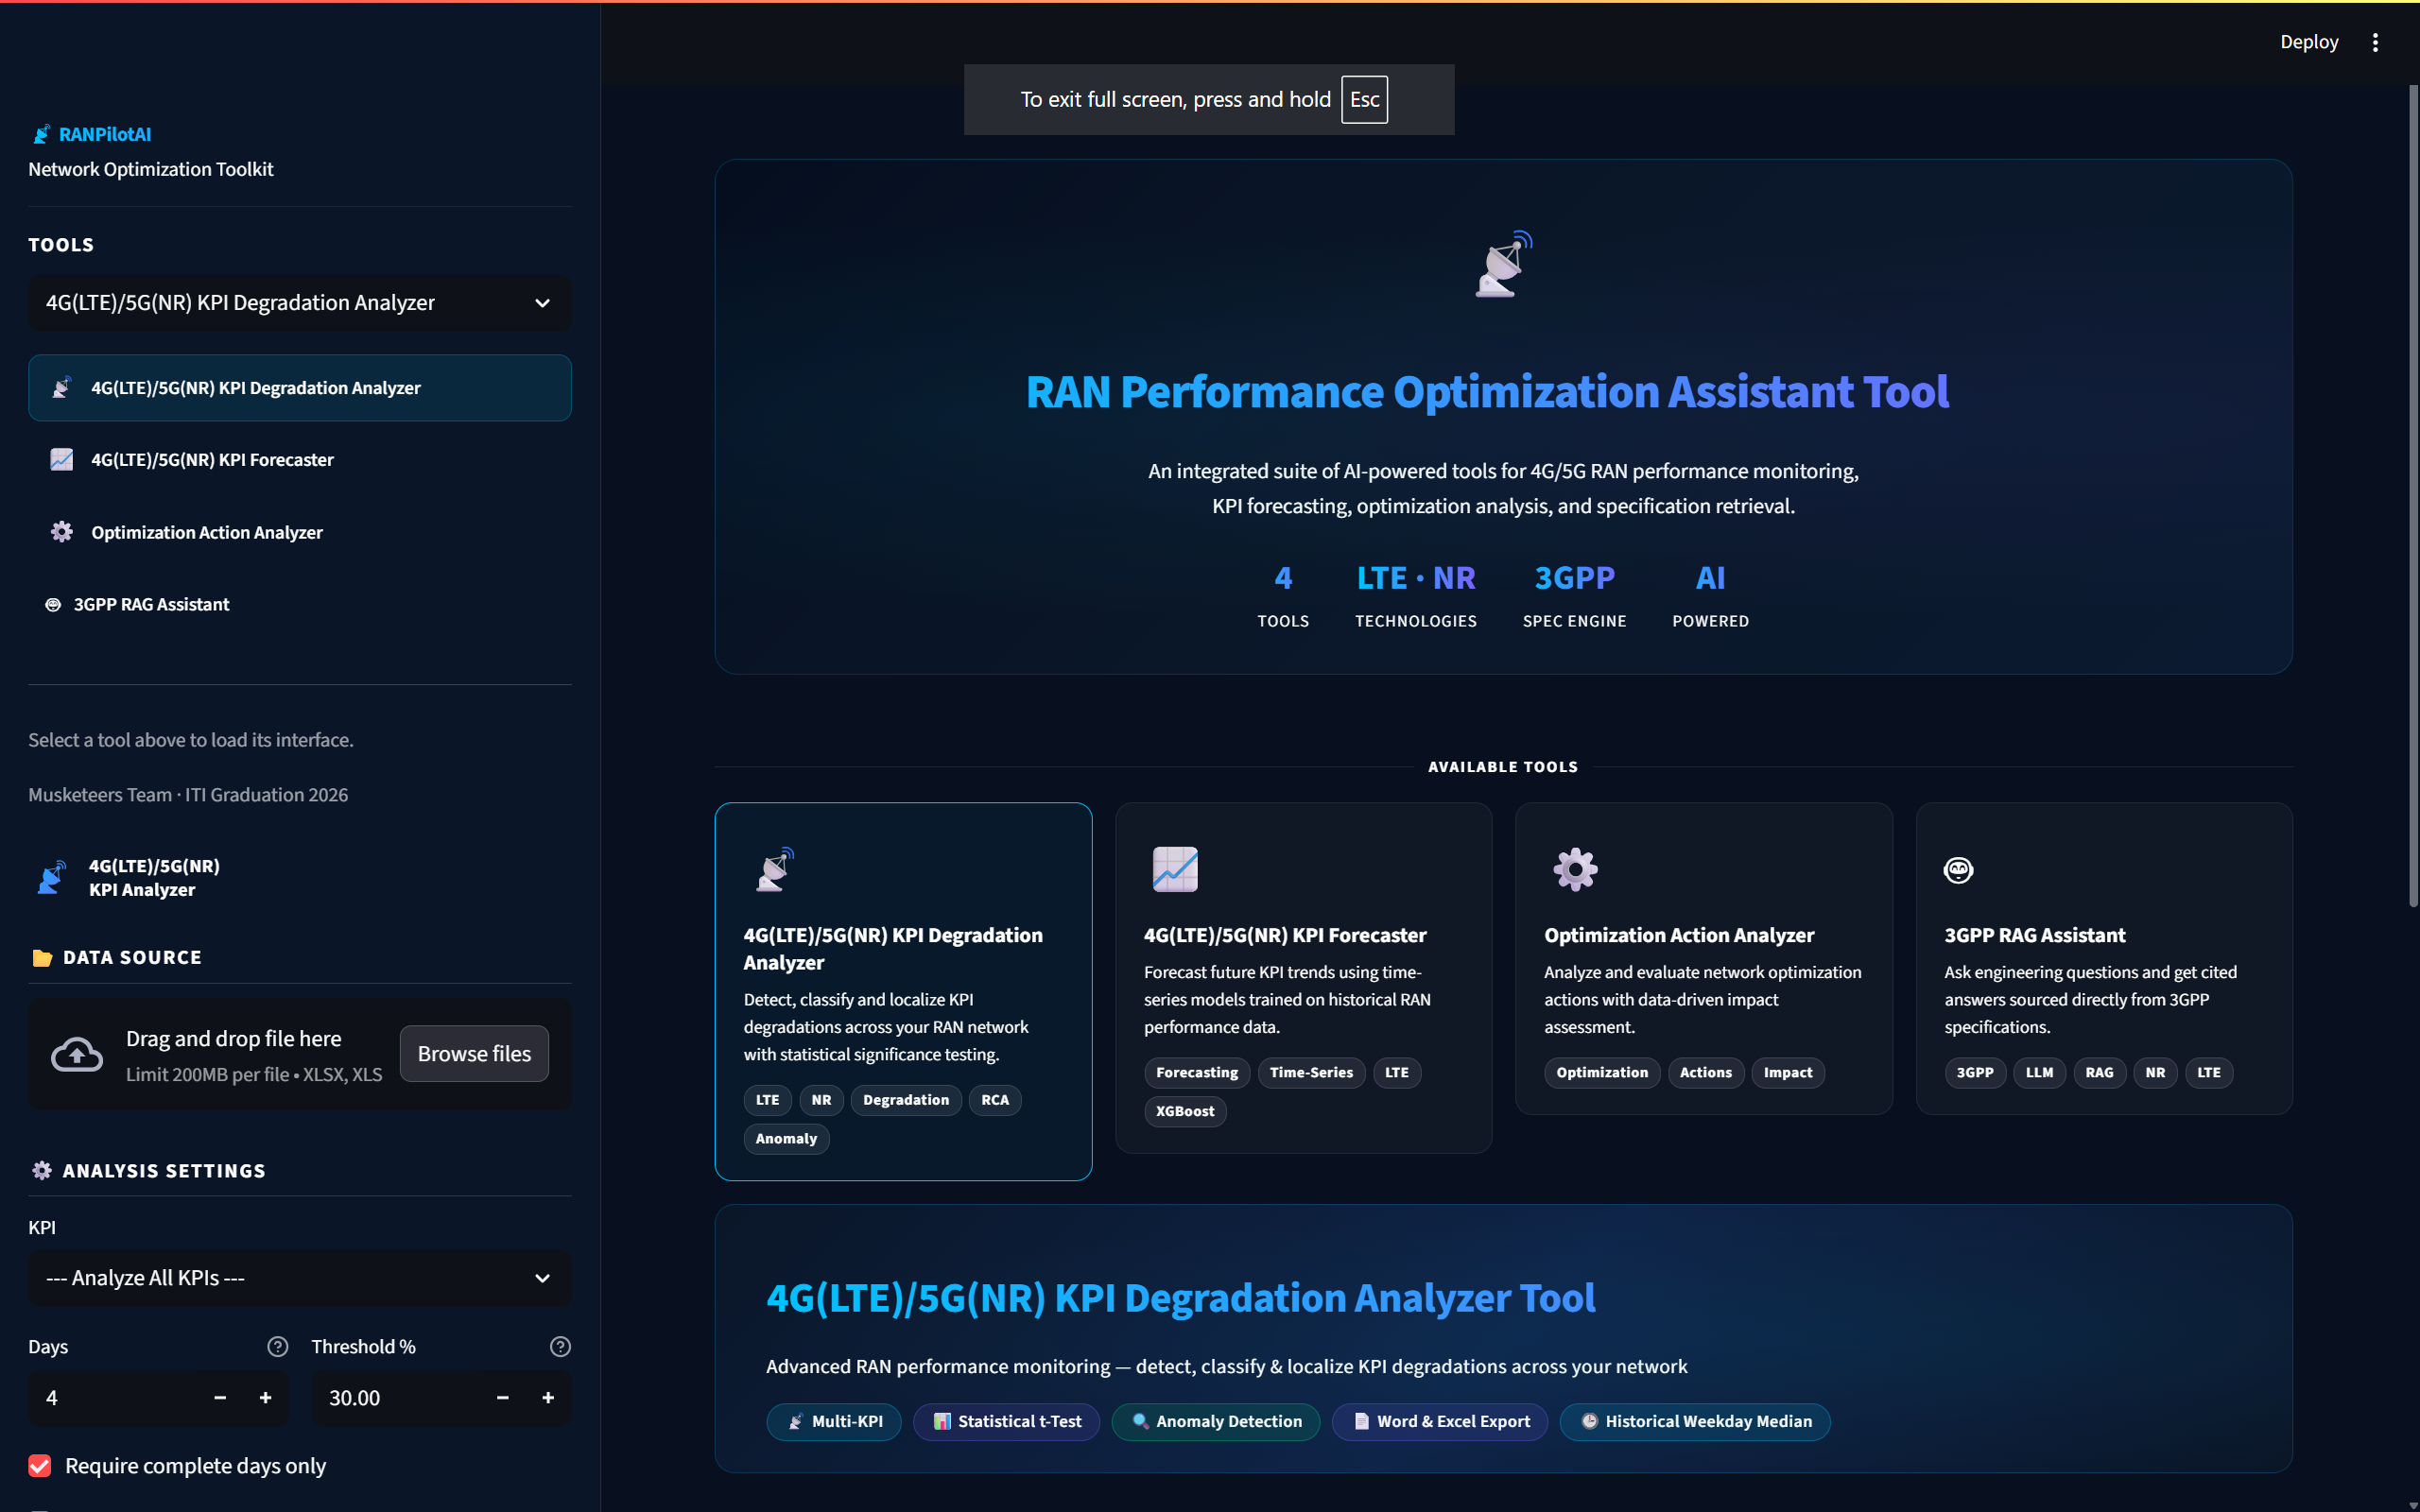
\includegraphics[width=\textwidth]{figures/chapter03/tool_navigation.png}
    \caption{Navigation interface of the RANPilotAI Telecom Hub presenting the four selectable analytical modules. The interface provides consistent access to KPI Degradation Analyzer, KPI Forecasting Engine, Optimization Action Analyzer, and Telecom RAG Assistant through a unified module selection paradigm.}
    \label{fig:tool_navigation}
\end{figure}

%%%%%%%%%%%%%%%%%%%%%%%%%%%%%%%%%%%%%%%%%%%%%%%%%%%%%%%%%%%%%%%%%%%%%%%%%%%%%%%%
\section{Design Objectives and Constraints}

\subsection{Functional Objectives}

The platform must support the complete RAN optimization workflow within a single environment. This includes uploading and validating KPI counter exports, configuring analysis parameters, executing degradation detection and forecasting computations, visualising results through interactive charts and tables, correlating configuration changes with KPI impact, and consulting 3GPP Technical Specifications using natural language queries. Each analytical module must operate independently while sharing common data services and presenting results through a consistent interface paradigm.

\subsection{Non-Functional Objectives}

The platform must be accessible through a standard web browser without requiring client-side software installation, operate on a single workstation without distributed computing infrastructure, and maintain interactive response times for UI operations. Analysis computations that require significant processing time must provide progress indication and allow cancellation. Data persistence must ensure that analysis results are retained across sessions, and export functionality must support integration with existing operational reporting workflows.

\subsection{Technical Constraints}

The platform is constrained to Python 3.11 for implementation consistency across all modules. Third-party dependencies are limited to packages available through standard Python package repositories with permissive licensing. The deployment target is a single Windows or Linux workstation with 16 GB RAM and a multi-core processor, sufficient to process datasets containing up to one million rows and five hundred columns without requiring cloud infrastructure or distributed computing frameworks.

%%%%%%%%%%%%%%%%%%%%%%%%%%%%%%%%%%%%%%%%%%%%%%%%%%%%%%%%%%%%%%%%%%%%%%%%%%%%%%%%
\section{Overall Platform Architecture}

The RANPilotAI platform follows a layered modular architecture comprising four principal components: the Telecom Hub, which coordinates user interaction and module routing; the Engineering Modules, which implement the four analytical capabilities; the Shared Components, which provide common functionality reused across modules; and the Platform Resources, which manage data persistence, configuration, and external service integration.

The Telecom Hub functions as the central access point. Rather than interacting directly with individual processing engines, users communicate exclusively with the hub, which manages application routing, session handling, and interaction with underlying analytical components. This centralised execution model simplifies software maintenance, reduces coupling between modules, and establishes a consistent execution model throughout the platform.

The Engineering Modules operate as independent subsystems connected through the Telecom Hub via standardized interfaces. Each module encapsulates its own processing logic, data models, and visualisation components while relying on shared components for common operations such as file upload handling, progress indication, and result export.

\begin{table}[H]
    \centering
    \caption{Platform components and their primary responsibilities within the RANPilotAI architecture.}
    \label{tab:platform_modules}
    \begin{tabular}{|p{3.5cm}|p{8cm}|}
        \hline
        \textbf{Component} & \textbf{Responsibilities} \\
        \hline
        Telecom Hub & Module routing, session management, unified navigation, shared UI components \\
        \hline
        KPI Degradation Analyzer & Data quality validation, degradation detection, RF-aware root cause analysis, export generation \\
        \hline
        KPI Forecasting Engine & Time-series decomposition, feature engineering, model training and evaluation, forecast generation \\
        \hline
        Optimization Action Analyzer & Configuration tracking, action hunk generation, KPI impact quantification, timeline visualisation \\
        \hline
        Telecom RAG Assistant & PDF processing, semantic indexing, vector retrieval, re-ranking, LLM prompt construction \\
        \hline
        Shared Components & File handling, progress indication, data export utilities, logging and error management \\
        \hline
        Platform Resources & Dolt database, vector store, configuration files, exported results persistence \\
        \hline
    \end{tabular}
\end{table}

Table~\ref{tab:platform_modules} summarises the platform components and their primary responsibilities. The separation between engineering modules and shared infrastructure ensures that analytical logic can evolve independently of platform services, while the centralised hub ensures that users experience a consistent interface across all modules.

%%%%%%%%%%%%%%%%%%%%%%%%%%%%%%%%%%%%%%%%%%%%%%%%%%%%%%%%%%%%%%%%%%%%%%%%%%%%%%%%
\section{Software Architecture and Design Patterns}

\subsection{Layered Architecture}

The platform adopts a layered architecture that separates user interaction, application logic, engineering modules, and data management into distinct software layers \cite{sommerville2015}. The presentation layer is implemented through Streamlit components and custom CSS styling, providing responsive layout management and interactive visualisations. The application logic layer contains the Telecom Hub orchestration code, session management, and module routing logic. The engineering module layer contains the analytical processing pipelines for each module. The data management layer abstracts database access, file system operations, and external service communication.

This separation improves maintainability by ensuring that each layer is responsible for a well-defined set of functionalities while communicating only with adjacent layers. Changes to the user interface do not affect analytical processing logic, and modifications to data storage mechanisms do not require changes to module orchestration code.

\subsection{Design Patterns}

The platform implements several established design patterns to improve code organisation and extensibility \cite{gamma1994}.

The Strategy pattern is applied to model selection in the KPI Forecasting Engine, allowing new forecasting models to be incorporated through a common evaluation interface. Each model implements the standard interface methods — \texttt{train}, \texttt{predict}, and \texttt{evaluate} — enabling the model selection protocol to compare arbitrary candidate models without conditional logic.

The Observer pattern supports real-time progress reporting during long-running analyses. Each analytical module emits progress events during computation, which the Telecom Hub captures and forwards to the Streamlit UI for display. This decouples analysis progress tracking from the specific implementation of each module.

The Facade pattern simplifies module interaction by presenting a consistent API surface to the Telecom Hub. Each engineering module exposes a standard set of entry points — \texttt{load\_data}, \texttt{configure}, \texttt{run\_analysis}, and \texttt{get\_results} — which the hub invokes without requiring knowledge of the module's internal processing pipeline.

\subsection{Data Flow Architecture}

The overall data flow within the RANPilotAI platform follows a unidirectional pipeline pattern. User inputs are captured by the Telecom Hub and forwarded to the selected engineering module. The module processes the input through its analytical pipeline, persisting intermediate results to the platform data layer. Completed results are returned to the hub for presentation through the Streamlit interface. Export operations are triggered by user request and routed to the appropriate export generator.

This architecture ensures that data flows in a single direction, simplifying debugging and ensuring that analysis state is fully reproducible from the original input data and configuration parameters.

%%%%%%%%%%%%%%%%%%%%%%%%%%%%%%%%%%%%%%%%%%%%%%%%%%%%%%%%%%%%%%%%%%%%%%%%%%%%%%%%
\section{Technology Stack}

\subsection{Backend Framework}

The platform is implemented in Python 3.11, selected for its extensive scientific computing ecosystem, strong type annotation support, and widespread adoption in data engineering and machine learning communities. The Streamlit framework provides the web-based user interface, offering rapid development of interactive data applications through a declarative programming model. Streamlit's automatic reloading, session state management, and component library accelerate frontend development while maintaining acceptable performance for the platform's analytical workloads.

\subsection{Data Processing}

Pandas provides the primary data manipulation infrastructure, supporting the loading, transformation, and aggregation of KPI datasets containing hundreds of columns and millions of rows. NumPy underpins numerical computations including statistical tests, rolling window operations, and matrix algebra required for feature engineering and model evaluation. The platform leverages Pandas' datetime indexing and groupby operations extensively for time-series analysis and weekday-matched baseline computation.

\subsection{Machine Learning}

Scikit-learn provides preprocessing utilities, evaluation metrics, and baseline model implementations used across multiple modules. XGBoost implements the gradient boosting regression models used in the KPI Forecasting Engine, providing efficient training through histogram-based algorithm variants and GPU acceleration support. Statsmodels provides the Holt-Winters exponential smoothing implementation and statistical test functions including Welch's t-test.

\subsection{Retrieval-Augmented Generation}

Sentence-transformers provides the BGE-large embedding model used to convert text chunks and user queries into dense vector representations. Qdrant serves as the local vector database, storing indexed document embeddings and supporting semantic similarity search with metadata filtering. The CrossEncoder from the sentence-transformers library implements the neural re-ranking stage, rescoring initial retrieval candidates to improve precision. OpenRouter provides unified API access to large language models including Llama and Gemma variants, enabling the platform to generate engineering responses grounded in retrieved specification excerpts.

\subsection{Data Persistence}

Dolt provides version-controlled SQL database functionality, enabling the Optimization Action Analyzer to track configuration commit history, query historical KPI snapshots, and compute before/after comparisons using Git-like branching and diff semantics. SQLite serves as the default persistence backend for smaller datasets and configuration state, while Parquet files provide efficient columnar storage for large KPI exports. The platform uses Apache ECharts through the Streamlit native charting interface for interactive visualisations.

%%%%%%%%%%%%%%%%%%%%%%%%%%%%%%%%%%%%%%%%%%%%%%%%%%%%%%%%%%%%%%%%%%%%%%%%%%%%%%%%
\section{Data Management Strategy}

\subsection{KPI Data Schema}

The platform defines a canonical KPI data schema that maps vendor-specific counter names to standardised internal identifiers. This schema normalises column naming conventions, units, and measurement directions across different network management system exports, enabling the analytical modules to operate on heterogeneous data sources without modification. The schema includes metadata for each KPI category specifying the performance pillar, measurement direction, theoretical bounds, and associated root cause detection rules.

\subsection{Configuration Change Tracking}

The Optimization Action Analyzer implements a configuration change tracking system built on Dolt's versioning semantics. Each configuration modification — including antenna tilt adjustments, transmit power changes, and handover parameter updates — is recorded as a Dolt commit with associated metadata specifying the cell identifier, parameter name, previous value, new value, timestamp, and author. This commit history enables the module to align configuration events with KPI time windows and compute the causal impact of individual changes or coordinated change campaigns.

\subsection{Vector Index Management}

The Telecom RAG Assistant maintains a persistent vector index of processed 3GPP specification documents. The indexing pipeline processes PDF files through text extraction, section-aware chunking, embedding generation, and vector storage. The index is rebuilt incrementally when specification documents are updated, ensuring that the retrieval corpus remains current with the latest 3GPP releases. Metadata associated with each chunk — including specification number, release version, section identifier, and page number — is stored alongside the embedding vector to support citation generation and specification filtering.

%%%%%%%%%%%%%%%%%%%%%%%%%%%%%%%%%%%%%%%%%%%%%%%%%%%%%%%%%%%%%%%%%%%%%%%%%%%%%%%%
\section{Module Interfaces and Integration}

\subsection{Telecom Hub Interface}

The Telecom Hub defines a standard module interface contract that each analytical module must implement. The contract specifies four principal methods: \texttt{load\_data} for ingesting user-uploaded files, \texttt{configure} for applying user-specified analysis parameters, \texttt{run\_analysis} for executing the analytical pipeline, and \texttt{get\_results} for retrieving completed analysis outputs. Additional optional methods support progress reporting, cancellation, and result export.

This interface contract enables the hub to orchestrate module execution through a uniform mechanism regardless of the specific analytical processing implemented within each module. New modules can be integrated by implementing the standard interface without modifying hub orchestration logic.

\subsection{Session State Management}

Streamlit's session state mechanism provides the foundation for multi-module workflow continuity. Each module maintains its own session state namespace, storing loaded data, configuration parameters, analysis results, and visualisation selections. The Telecom Hub coordinates module switching by preserving session state across module transitions, enabling engineers to perform degradation analysis, switch to the forecasting module to predict future trajectories, and return to the degradation module with analysis context intact.

\subsection{Data Sharing Between Modules}

The platform supports controlled data sharing between modules through the platform's shared data layer. The KPI Degradation Analyzer can export degraded cell lists that serve as input to the KPI Forecasting Engine, enabling engineers to focus forecasting computation on cells that have already been identified as degraded. Similarly, the Optimization Action Analyzer can reference degraded cell identifiers from the degradation module to focus configuration impact analysis on cells experiencing active performance issues.

%%%%%%%%%%%%%%%%%%%%%%%%%%%%%%%%%%%%%%%%%%%%%%%%%%%%%%%%%%%%%%%%%%%%%%%%%%%%%%%%
\section{Deployment Architecture}

\subsection{Single-Workstation Deployment}

The platform is designed for deployment on a single workstation without distributed computing infrastructure. The Streamlit web server runs locally, serving the user interface through a web browser on the same machine or on connected devices within the local network. This deployment model prioritises simplicity, portability, and data locality — all KPI data and analysis results remain on the operator's workstation, addressing data security and regulatory compliance requirements.

\subsection{Scalability Considerations}

While the current deployment model operates on a single workstation, the modular architecture enables horizontal scaling without architectural redesign. Each analytical module can be deployed as an independent service communicating with the Telecom Hub through network APIs, allowing compute-intensive modules to be hosted on dedicated servers while maintaining the unified user interface. The version-controlled data backend provided by Dolt supports multi-user collaboration through its branching and merging semantics, enabling teams of engineers to work on parallel analysis investigations without interfering with each other's data.

%%%%%%%%%%%%%%%%%%%%%%%%%%%%%%%%%%%%%%%%%%%%%%%%%%%%%%%%%%%%%%%%%%%%%%%%%%%%%%%%
\section{Summary}

This chapter has presented the overall system design of the RANPilotAI platform. The platform adopts a modular, layered architecture in which four independent analytical modules operate within a unified web-based engineering environment coordinated by the Telecom Hub. The design prioritises modularity, maintainability, usability, and extensibility, ensuring that the platform can evolve to incorporate new analytical capabilities without architectural redesign.

The technology stack combines established open-source libraries for data processing, machine learning, retrieval-augmented generation, and web-based user interface development. The data management strategy provides persistent, version-controlled storage for KPI datasets, configuration histories, and document indices. The module integration architecture defines standardised interfaces that enable the Telecom Hub to orchestrate analytical workflows across heterogeneous processing engines.

The subsequent chapters describe each analytical module in detail. Chapter~\ref{chap:kpi_degradation} presents the KPI Degradation Analyzer, Chapter~\ref{ch:forecasting} presents the KPI Forecasting Engine, Chapter~\ref{chap:opt-action-analyzer} presents the Optimization Action Analyzer, and Chapter~\ref{chap:telecom_rag} presents the Telecom RAG Assistant. Each chapter follows the structure established in Chapter~\ref{chap:introduction}: module introduction, operational motivation, technical problem formulation, background theory, configuration and results presentation, and summary.
